% Created 2019-07-22 Mon 13:37
% Intended LaTeX compiler: pdflatex
\documentclass[presentation,aspectratio=169,smaller]{beamer}
\usepackage[utf8]{inputenc}
\usepackage[T1]{fontenc}
\usepackage{graphicx}
\usepackage{grffile}
\usepackage{longtable}
\usepackage{wrapfig}
\usepackage{rotating}
\usepackage[normalem]{ulem}
\usepackage{amsmath}
\usepackage{textcomp}
\usepackage{amssymb}
\usepackage{capt-of}
\usepackage{hyperref}
\usepackage{color}
\usepackage[newfloat]{minted}
\usemintedstyle{tango}
\setminted{fontsize=\scriptsize}
\setminted{mathescape=true}
\setbeamertemplate{itemize items}[circle]
\setbeamertemplate{enumerate items}[default]
\usetheme{default}
\author{Boris Buliga, Valentyn Vakatsiienko}
\date{\today}
\title{Functional Workshop: Part 1}
\hypersetup{
 pdfauthor={Boris Buliga, Valentyn Vakatsiienko},
 pdftitle={Functional Workshop: Part 1},
 pdfkeywords={},
 pdfsubject={},
 pdfcreator={Emacs 27.0.50 (Org mode 9.2.4)}, 
 pdflang={English}}
\begin{document}

\maketitle

\section*{Intro}
\label{sec:orgf09023e}

\begin{frame}[label={sec:org337d2d9}]{About us}
\begin{block}{Valik}
Server guild manager in Kyiv. Formerly forced people to use functional
programming style in the Domains (Premium) team. Now works on Tagless Infra to
provide you with the best tools for your daily needs. Which are all functional,
of course.

\pause
\end{block}

\begin{block}{Boris}
Developer at Payments by Wix team. Jumps between two extremes - Emacs Lisp and
Haskell. Wants to force people around to use both languages, but can't explain
why.
\end{block}
\end{frame}

\begin{frame}[label={sec:org0a1242e}]{About the Workshop}
\begin{itemize}
\item Basic workshop is split into 3 parts:
\begin{enumerate}
\item Type classes, Semigroups and Monoids.
\item Functors and Applicative Functors.
\item Monads.
\end{enumerate}
\item Theory and practice. You'll have to write code, so make sure your laptop is
ready for this.
\item Main target audience is Scala developers.
\item Workshop is duplicated in Haskell.
\end{itemize}
\end{frame}

\begin{frame}[label={sec:orgd4579f1},fragile]{Whys}
 \begin{itemize}
\item Functional programming roams (a bit).
\begin{itemize}
\item More projects are using functional programming techniques and idioms (at
different scale).
\end{itemize}
\item Some people are still confused by all these functional talks (\texttt{OptionT}, type
lambdas etc).
\item Having a common language and understanding of some fundamental stuff is
important.
\end{itemize}
\end{frame}

\begin{frame}[label={sec:org3dd0b88}]{Plan}
\begin{itemize}
\item Type classes
\item Property based testing (just a tip of)
\item Semigroups
\item Monoids
\item 3 interesting™ tasks
\end{itemize}
\end{frame}

\section*{Typeclasses}
\label{sec:org62ce570}

\begin{frame}[label={sec:orge441282}]{Fulfilling a dream}
\begin{itemize}
\item Imagine that we are game developers (yay!).
\item Imagine that we are writing a game (double yay!).
\item And every game needs a hero, who can properly introduce itself.
\end{itemize}
\end{frame}

\begin{frame}[label={sec:org7dad0e7},fragile]{Meet the hero}
 \begin{minted}[]{scala}
case class Hero(name: String, job: String, level: Int) {
  def introduce(): String = s"Hi! My name is $name. I am $level level $job."
}

object Game extends App {
  val player = Hero("Valik", "Black Mage", 20)

  println(player.introduce())
}

// Hi! My name is Valik. I am 20 level Black Mage.
\end{minted}
\end{frame}

\begin{frame}[label={sec:orgadf568f},fragile]{Every hero needs a monster}
 \begin{minted}[]{scala}
case class Hero(name: String, job: String, level: Int) {
  def introduce(): String = s"Hi! My name is $name. I am $level level $job."
}

case class Orc(name: String, level: Int) {
  def introduce(): String =
    s"Lok-tar ogar! Me be $name. Me be strong. Level $level strong!"
}

case class Ooze(level: Int) {
  def introduce(): String = 1.to(level).map(_=>"brlup").mkString("-")
}

object Game extends App {
  val player = Hero("Valik", "Black Mage", 20)
  val orc = Orc("Garrosh", 105)
  val ooze = Ooze(2)

  println(player.introduce())
  println(orc.introduce())
  println(ooze.introduce())
}

// Hi! My name is Valik. I am 20 level Black Mage.
// Lok-tar ogar! Me be Garrosh. Me be strong. Level 105 strong!
// brlup-brlup
\end{minted}
\end{frame}

\begin{frame}[label={sec:org2b4c5db},fragile]{Everyone is polite}
 \begin{itemize}
\item In our world everyone is polite. Even ooze, brlup-blup!
\item Rendering process of greetings is a hard process and boils down to the string
manipulation.
\item So we decided to avoid code repetition and write a function that does just that.

\begin{minted}[]{scala}
object Game extends App {
  def introduce(phrase: String): Unit = {
    // some real shit animations
    println(phrase)
    // some real shit animations
  }
  introduce(hero.introduce())
  introduce(orc.introduce())
  introduce(ooze.introduce())
}
\end{minted}

\item But it would so nice to avoid all this \texttt{\_.introduce()}.
\begin{itemize}
\item And you know, DRY leads to disasters!
\end{itemize}
\end{itemize}
\end{frame}

\begin{frame}[label={sec:org3a6aedb},fragile]{Introducing abstractions}
 \begin{minted}[]{scala}
trait Introducible {
  def introduce(): String
}

case class Hero(name: String, job: String, level: Int) extends Introducible {
  override def introduce(): String = s"Hi! My name is $name. I am $level level $job."
}

case class Orc(name: String, level: Int) extends Introducible {
  override def introduce(): String =
    s"Lok-tar ogar! Me be $name. Me be strong. Level $level strong!"
}

case class Ooze(level: Int) extends Introducible {
  override def introduce(): String = 1.to(level).map(_=>"brlup").mkString("-")
}
\end{minted}
\end{frame}

\begin{frame}[label={sec:org8d418a5},fragile]{Using the \texttt{trait}}
 \begin{minted}[]{scala}
object Game extends App {
  val player = Hero("Valik", "Black Mage", 20)
  val orc = Orc("Garrosh", 105)
  val ooze = Ooze(2)

  def introduce(creatute: Introducible): Unit = {
    // some real shit animations
    println(creatute.introduce())
    // some real shit animations
  }

  introduce(player)
  introduce(orc)
  introduce(ooze)
}

// Hi! My name is Valik. I am 20 level Black Mage.
// Lok-tar ogar! Me be Garrosh. Me be strong. Level 105 strong!
// brlup-brlup
\end{minted}
\end{frame}

\begin{frame}[label={sec:org6b3475e},fragile]{Here comes the cockatrice}
 \begin{minted}[]{scala}
import io.proprietary.monsters.cockatrice._

/*...*/

object Game extends App {
  /*...*/

  val cockatrice = Cockatrice(level = 666, element = Element.Fire)

  introduce(cockatrice) // ???
                        // ain't gonna work
}
\end{minted}
\end{frame}

\begin{frame}[label={sec:org5822e17},fragile]{Shawarma to the rescue}
 \begin{columns}
\begin{column}{0.25\columnwidth}
\begin{center}

\includegraphics[height=7cm]{images/shawarma.jpg}
\end{center}
\end{column}

\begin{column}{0.75\columnwidth}
\begin{minted}[]{scala}
import io.proprietary.monsters.cockatrice._

/*...*/

case class CockatriceWrapper(cockatrice: Cockatrice) extends Introducible {
  override def introduce(): String = {
    import cockatrice._
    s"Haha. I am a ${element.shortName} cockatrice of level ${level}."
  }
}

object Game extends App {
  /*...*/

  val cockatrice = Cockatrice(level = 666, element = Element.Fire)
  val cockatriceW = CockatriceWrapper(cockatrice)

  introduce(cockatriceW)

  /*...*/
}


// Haha. I am a fire cockatrice of level 666.
\end{minted}
\end{column}
\end{columns}
\end{frame}

\begin{frame}[label={sec:org1c58c5e}]{Properties we care about}
\begin{itemize}
\item Abstraction - we care about what you can do and not what you are.
\item Composition - we want a way to express that we want something that can do
several things at once.
\item Extensibility - we want to extend even types that we don’t own. Built-in types
as well.
\end{itemize}
\end{frame}

\begin{frame}[label={sec:orgce6abd8},fragile]{With \texttt{trait} + wrappers approach}
 \begin{itemize}
\item Abstraction works. We are able to define generic \texttt{introduce} function.
\item Composition works thanks to \texttt{with} keyword. But it's not commutative.
\begin{minted}[]{scala}
def surpriseAttack[A <: Introducible with CanAttack](creature: A): Unit
\end{minted}
\item Extensibility is possible with some caveats:
\begin{itemize}
\item No consistency - we wrap only types we don't own.
\item Nightmare to maintain when you need several behaviours. So you wrap the
wrapper.
\item Bad usability - you can’t interchangeably use wrapper and the underlying
value.
\end{itemize}
\end{itemize}

\pause

You know where it’s going to, right?
\end{frame}

\begin{frame}[label={sec:org4002be2}]{F[\_]}
\begin{center}

\includegraphics[height=7cm]{images/f_.jpg}
\end{center}
\end{frame}

\begin{frame}[label={sec:org8699db2},fragile]{What if\ldots{}}
 We divide data and behaviour

\pause

\begin{columns}
\begin{column}[t]{0.42\columnwidth}
\begin{minted}[]{scala}
trait Introducible {
  def introduce(): String
}
\end{minted}
\end{column}

\begin{column}[t]{0.05\columnwidth}
\vspace*{0px}

{\large \Rightarrow}
\end{column}

\begin{column}[t]{0.55\columnwidth}
\begin{minted}[]{scala}
trait Introducible[A] {
  def introduce(a: A): String
}
\end{minted}

\begin{itemize}
\item \texttt{A} is data
\item \texttt{Introducible[A]} - behaviour
\end{itemize}
\end{column}
\end{columns}

\pause

\vspace*{1cm}

So we can pass separately two values:

\begin{itemize}
\item data itself
\item implementation of behaviour
\end{itemize}

\pause

\begin{columns}
\begin{column}[t]{0.42\columnwidth}
\begin{minted}[]{scala}
def introduce(creatute: Introducible): Unit =
  println(creatute.introduce())
\end{minted}
\end{column}

\begin{column}[t]{0.05\columnwidth}
\vspace*{0px}

{\large \Rightarrow}
\end{column}

\begin{column}[t]{0.55\columnwidth}
\begin{minted}[]{scala}
def introduce[A](creature: A)(impl: Introducible[A]): Unit =
  println(impl.introduce(creature))
\end{minted}
\end{column}
\end{columns}
\end{frame}

\begin{frame}[label={sec:orgad04d9f},fragile]{We treat our own types}
 \begin{minted}[]{scala}
trait Introducible[A] {
  def introduce(a: A): String
}

case class Hero(name: String, job: String, level: Int)

object Hero {
  val introducibleHero: Introducible[Hero] = (a: Hero) => {
    import a._
    s"Hi! My name is $name. I am $level level $job."
  }
}

object Game extends App {
  def introduce[A](creature: A)(ev: Introducible[A]): Unit =
    println(ev.introduce(creature))

  introduce(Hero(name = "Valik", job = "Black Mage", level = 20))(Hero.introducibleHero)
}
\end{minted}
\end{frame}

\begin{frame}[label={sec:org1dc9974},fragile]{And external types in the same way}
 \begin{minted}[]{scala}
import io.proprietary.monsters.cockatrice._

trait Introducible[A] {
  def introduce(a: A): String
}

object Introducible {
  val introducibleCockatrice: Introducible[Cockatrice] = (a: Cockatrice) => {
    s"Haha. I am a ${a.element.shortName} cockatrice of level ${a.level}."
  }
}

object Game extends App {
  def introduce[A](creature: A)(ev: Introducible[A]): Unit = println(ev.introduce(creature))

  introduce(Cockatrice(level = 666, element = Element.Fire))(Introducible.introducibleCockatrice)
}
\end{minted}
\end{frame}

\begin{frame}[label={sec:org500af56}]{But passing implementation around is\ldots{}}
\begin{center}

\includegraphics[height=7cm]{images/cucumber.jpg}
\end{center}

Cucumbersome
\end{frame}

\begin{frame}[label={sec:orgb53468c},fragile]{So implicits :(}
 \begin{minted}[]{scala}
object Introducible {
  implicit val introducibleCockatrice: Introducible[Cockatrice] = /*...*/
}

object Hero {
  implicit val introducibleHero: Introducible[Hero] = /*...*/
}

object Game extends App {
  def introduce[A](creature: A)(implicit ev: Introducible[A]): Unit =
    println(ev.introduce(creature))

  introduce(Hero(name = "Valik", job = "Black Mage", level = 20))
  introduce(Cockatrice(level = 666, element = Element.Fire))
}
\end{minted}
\end{frame}

\begin{frame}[label={sec:org136ced0},fragile]{Summoning the summoner}
 \begin{minted}[]{scala}
trait Introducible[A] { /*...*/ }

object Introducible {
  def apply[A: Introducible]: Introducible[A] = implicitly[Introducible[A]]

  /*...*/
}

/*...*/

object GameSummoner extends App {
  def introduce[A: Introducible](creature: A): Unit =
    println(Introducible[A].introduce(creature))

  introduce(Hero(name = "Valik", job = "Black Mage", level = 20))
  introduce(Cockatrice(level = 666, element = Element.Fire))
}
\end{minted}
\end{frame}

\begin{frame}[label={sec:orgc150a87},fragile]{So with type classes}
 \begin{itemize}
\item Abstraction works. Again, we are able to define generic \texttt{introduce} function.
\item Composition works, just require two behaviours.
\begin{minted}[]{scala}
object Game {
  def surpriseAttack[A : Introducible : CanAttack](creatute: A): Unit
}
\end{minted}
\item Extensibility achieved and maintained consistency and usability.
\begin{itemize}
\item Consistent - we treat our own types the same way we types we don't own.
\item Usability - no wrappers, no interchangeably problem. You pass data and
behaviour implementation separately.
\end{itemize}
\end{itemize}
\end{frame}

\begin{frame}[label={sec:org61835b7}]{So type classes}
Type class is just a construct that supports \alert{ad hoc polymorphism}. E.g. allows
one to define polymorphic functions that can be applied to arguments of
different types and behave differently based the type of the arguments.

In other words, function overloading.

In Scala this can be achieved in several ways:

\begin{itemize}
\item Class inheritance or traits.
\item Type classes (traits + implicits).
\end{itemize}
\end{frame}

\section*{Semigroup}
\label{sec:org990ad58}

\begin{frame}[label={sec:orgbe9a39c}]{Semigroup}
A semigroup is an algebraic structure consisting of a set together with an
associative binary operation.

\pause

A semigroup is a set \(S\) with binary operation \(\cdot : S \times S \rightarrow
S\) that satisfies associativity property:

$$\forall a, b, c \in S : (a \cdot b) \cdot c = a \cdot (b \cdot c)$$

\pause

\alert{Important}. Semigroup is a pair of the set and the operation. You can’t say
 that string is a semigroup, you must provide an operation. And in many cases
 there is more than one operation for a set to form a semigroup.

\pause

\alert{Note}. We usually omit the requirement that operation must be closed, e.g.
\(\forall a, b \in S : a \cdot b \in S\).
\end{frame}

\begin{frame}[label={sec:orgd0c8221},fragile]{But it’s not that scary}
 \begin{columns}
\begin{column}{0.5\columnwidth}
\begin{minted}[]{scala}
package object typeclass {

  //
  // Laws:
  //   1. $\forall a, b, c \in A: (a \cdot b) \cdot c = a \cdot (b \cdot c)$
  //
  trait Semigroup[A] {
    def append(x: A, y: A): A
  }

  object Semigroup {
    def apply[A: Semigroup]: Semigroup[A] =
      implicitly[Semigroup[A]]
  }

}
\end{minted}
\end{column}

\begin{column}{0.5\columnwidth}
\begin{center}

\includegraphics[height=7cm]{images/scary.png}
\end{center}
\end{column}
\end{columns}
\end{frame}

\begin{frame}[label={sec:orge0108df}]{Laws are important}
\begin{itemize}
\item In most cases type classes should have some associated laws.
\item Laws describe behaviour of the interface, what you can expect.
\item This gives you confidence when you combine pieces of code.
\end{itemize}
\end{frame}

\begin{frame}[label={sec:org2c3e81b},fragile]{Instance example}
 \begin{minted}[]{scala}
package object implicits {
  implicit val stringSemigroup: Semigroup[String] = new Semigroup[String] {
    override def append(x: String, y: String): String = x + y
  }
}
\end{minted}
\end{frame}

\begin{frame}[label={sec:orgfb023b8},fragile]{Checking laws - \sout{pen and paper} in comments}
 \begin{minted}[]{scala}
package object implicits {
  implicit val stringSemigroup: Semigroup[String] = new Semigroup[String] {
    override def append(x: String, y: String): String = x + y
  }
}

/*
append(a, append(b, c))
  = append(a, b + c)
  = a + (b + c)
  = (associativity of +)
  = (a + b) + c = append(a + b, c)
  = append(append(a, b), c)
*/
\end{minted}
\end{frame}

\begin{frame}[label={sec:org12870b0}]{You're programmer after all}
\begin{center}

\includegraphics[height=7cm]{images/you-re-programmer.jpg}
\end{center}
\end{frame}

\begin{frame}[label={sec:org9d938ff},fragile]{Question on the interview: property based testing}
 \begin{minted}[]{scala}
object SemigroupSpecification extends Properties("Semigroup") with SemigroupSpecificationSupport {
 include(semigroup[String](stringSemigroup))
}

trait SemigroupSpecificationSupport {
 def semigroup[A](sg: Semigroup[A])(implicit ar: Arbitrary[A], tag: ClassTag[A]): Properties =
   new Properties(s"Semigroup[${tag.toString}]") {
     // $\forall a, b, c \in A: (a \cdot b) \cdot c = a \cdot (b \cdot c)$
     property("associativity") = forAll { (a: A, b: A, c: A) =>
       sg.combine(sg.append(a, b), c) =? sg.append(a, sg.append(b, c))
     }
   }
}

/*
+ Semigroup.Semigroup[java.lang.String].associativity: OK, passed 100 tests
  .
*/
\end{minted}
\end{frame}

\begin{frame}[label={sec:org2319d22}]{More examples}
\begin{itemize}
\item Numbers with \(+\), \(*\), \(min\), \(max\)
\item Booleans with conjunction, disjunction, implication etc.
\item Square nonnegative matrices with multiplication.
\item Lists, Strings, Maps etc. with concatenation/union
\end{itemize}
\end{frame}

\begin{frame}[label={sec:orgd04373c}]{Contra-examples}
\begin{itemize}
\item \(\{\mathbb{N}, /\}\) is not a Semigroup, because \(/\) is not associative.
\item The same goes for \(\{\mathbb{N}, a^b \}\).
\item \(\{\mathbb{N}, -\}\) is not a Semigroup, because \(-\) is not a closed operation,
e.g. \(\exists a, b \in \mathbb{N}: a - b \notin \mathbb{N}\),
for example \(10 - 15 = -5 \notin \mathbb{N}\).
\end{itemize}
\end{frame}

\begin{frame}[label={sec:orgfa7c860},fragile]{Lets hack}
 \begin{enumerate}
\item Clone \texttt{git@github.com:d12frosted/wax.git}
\item Add missing definitions in \texttt{wax.typeclass.semigroup}
\item Run tests in \texttt{wax.typeclass.semigroup}
\end{enumerate}
\end{frame}

\section*{Monoid}
\label{sec:orgacaea69}

\begin{frame}[label={sec:orgfc3a53d}]{Monoid}
A monoid is an algebraic structure consisting of a set together with an
associative binary operation and an identity element from that set.

\pause

A monoid is a set \(S\) with binary operation \(\cdot : S \times S \rightarrow
S\) that satisfies associativity property:

$$\forall a, b, c \in S : (a \cdot b) \cdot c = a \cdot (b \cdot c)$$

and identity element \(e\) that satisfies

$$\forall a \in S : e \cdot a = a \cdot e = a$$

\pause

In other words, monoid is just a semigroup with identity element.
\end{frame}

\begin{frame}[label={sec:orgedbf3c8},fragile]{Again, it's not that scary}
 \begin{minted}[]{scala}
package object typeclass {

  //
  // Laws:
  //   1. $\forall a, b, c \in S : (a \cdot b) \cdot c = a \cdot (b \cdot c)$
  //   2. $\forall a \in S : e \cdot a = a \cdot e = a$
  //
  trait Monoid[A] extends Semigroup[A] {
    def empty: A
  }

  object Monoid {
    def apply[A: Monoid]: Monoid[A] = implicitly[Monoid[A]]
  }

}
\end{minted}
\end{frame}

\begin{frame}[label={sec:orgd35a6ea},fragile]{Examples}
 \begin{itemize}
\item \(\{\mathbb{N}_0, +\}\), where \(0\) is the identity element.
\item \(\{\mathbb{N}, *\}\), where \(1\) is the identity element.
\item Boolean with XOR, XNOR, OR, AND.
\item String with concatenation (empty string is identity element).
\end{itemize}

But not every Semigroup forms a Monoid (we are not talking about free monoids
here):

\begin{itemize}
\item \texttt{BigNumber} practically doesn’t have identity element for \texttt{min}.
\end{itemize}
\end{frame}

\section*{Transition to the practical part}
\label{sec:org3c1ecaf}

\begin{frame}[label={sec:orgfbd8726}]{The most important question}
\begin{center}
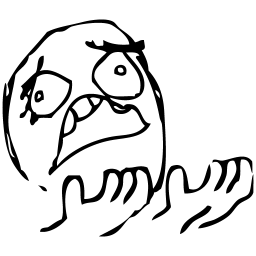
\includegraphics[height=7cm]{images/whyyy.png}
\end{center}

Why did we learn this?
\end{frame}

\section*{Fibonacci}
\label{sec:org97bf7fc}

\begin{frame}[label={sec:org9e25a74}]{The Fibonacci numbers}
On the interview we ask people to write a function that returns the nth
Fibonacci number.

\begin{align*}
  F_0 &= 0 \\
  F_1 &= 1 \\
  F_n &= F_{n - 1} + F_{n - 2}, \forall n > 1 \\
\end{align*}
\end{frame}

\begin{frame}[label={sec:orgc70ef5b},fragile]{Solution}
 \begin{columns}
\begin{column}[t]{0.5\columnwidth}
\begin{block}{What we expect}
\begin{minted}[]{scala}
def fib(n: Int): Int = {
  def fibTail(n: Int, a: Int, b: Int): Int = n match {
    case 0 => a
    case _ => fibTail(n - 1, b, a + b)
  }

  fibTail(n, 0, 1)
}
\end{minted}
\end{block}
\end{column}



\begin{column}[t]{0.5\columnwidth}
\begin{block}{Ideal solution}
\begin{align*}
  F_n &= \frac {\phi ^ n - {(- \phi)}^{-n}} {\sqrt{5}} \\
  &= \frac {\phi ^ n - {(- \phi)}^{-n}} {2\phi - 1} \\
  \\
  \phi &= \frac {1 + \sqrt{5}}{2}
\end{align*}

\pause
\end{block}
\end{column}
\end{columns}

As they say, truth is somewhere in the logarithm.
\end{frame}
\begin{frame}[label={sec:org200214d},fragile]{Two folds}
 \begin{itemize}
\item \texttt{def foldl[A, B](xs: Seq[A])(z: B)(op: B => A => B): B}
\begin{itemize}
\item Folds the structure from left to right
\end{itemize}
\item \texttt{def foldr[A, B](xs: Seq[A])(z: B)(op: A => B => B): B}
\begin{itemize}
\item Folds the structure from right to left
\end{itemize}
\item Since combining function is asymmetrical in its types:
\begin{itemize}
\item It’s impossible to place parentheses in the arbitrary fashion or even just
change the direction of the \texttt{fold}
\item It’s impossible to implement a total \texttt{fold} without default value of type \texttt{B}
\end{itemize}
\end{itemize}
\end{frame}

\begin{frame}[label={sec:org854bf18}]{Example}
\begin{columns}
\begin{column}[t]{0.5\columnwidth}
\begin{block}{foldl}
\begin{center}
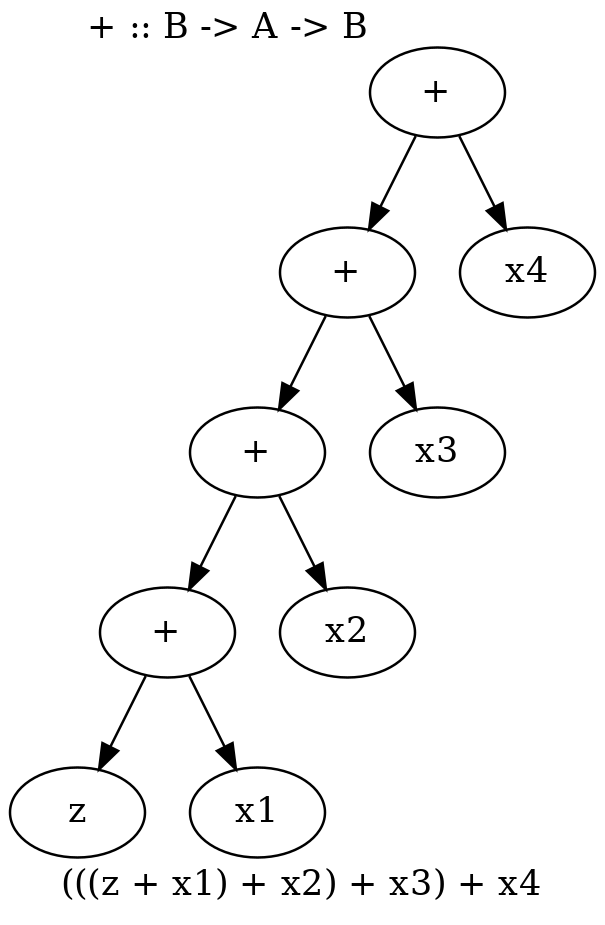
\includegraphics[height=6cm]{.dot/foldl-1.png}
\end{center}
\end{block}
\end{column}

\begin{column}[t]{0.5\columnwidth}
\begin{block}{foldr}
\begin{center}
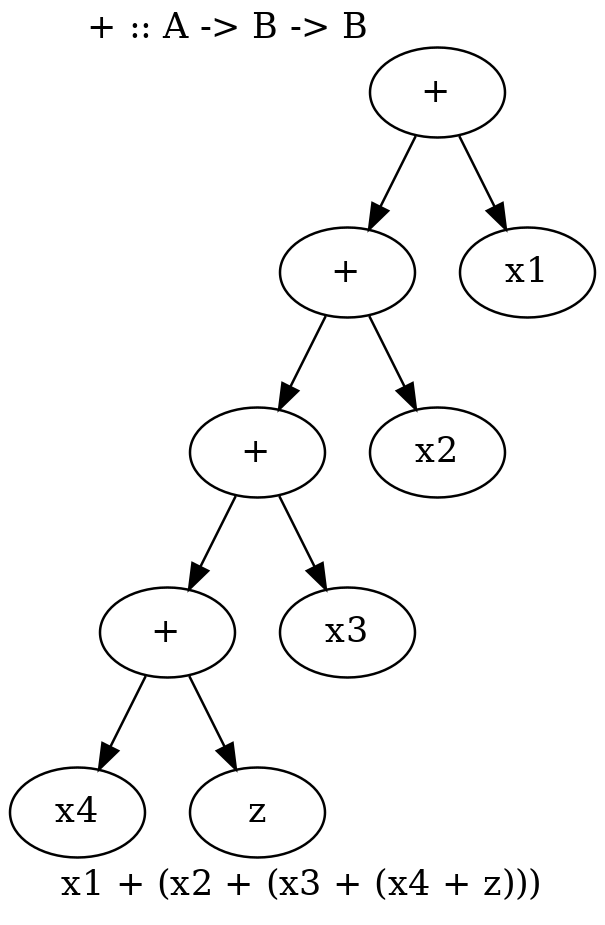
\includegraphics[height=6cm]{.dot/foldr-1.png}
\end{center}
\end{block}
\end{column}
\end{columns}
\end{frame}

\begin{frame}[label={sec:org7111aef},fragile]{What Monoid gives us}
 \begin{itemize}
\item Combining function is symmetrical (\texttt{append : A -> A -> A}).
\item Monoid provides identity element of type \texttt{A} (\texttt{empty}).
\item So we can define a special \texttt{fold}
\begin{itemize}
\item \texttt{def foldMonoid[A: Monoid](xs: Seq[A]): A}
\end{itemize}
\item Associativity law says that we can put parentheses in an arbitrary fashion.
\item Identity law says that we can place identity element anywhere - on the far
left, on the far right or even in the middle.
\item Laws that we checked are giving us means to abstract implementation.
\item When we ask consumer of our API to provide us a Monoid we don't want only a
behaviour but behaviour that follows the \alert{laws}. We want these \alert{properties} as
much as we want the functions.
\end{itemize}
\end{frame}

\begin{frame}[label={sec:org8980c3a}]{Power in terms of Monoid}
\begin{itemize}
\item In some cases all elements of the list are the same.
\pause
\begin{equation*}
  a + (a + (a + \ldots + a) \ldots ) = a ^ n
\end{equation*}
\end{itemize}

\pause

\begin{itemize}
\item Since we can reorder the parentheses, we can arrange them like this.
\end{itemize}

\pause
\begin{center}
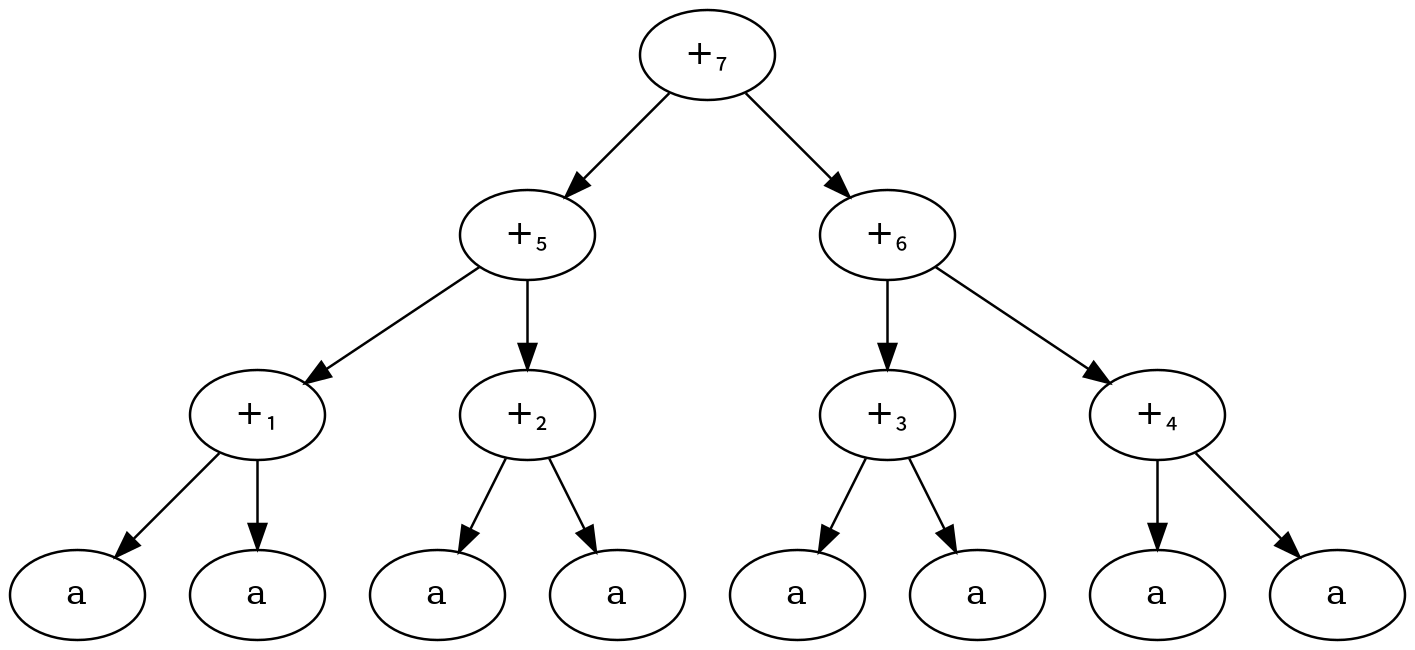
\includegraphics[height=4cm]{.dot/fold-power-1.png}
\end{center}
\end{frame}

\begin{frame}[label={sec:org437d800}]{Power in terms of Monoid}
\begin{center}
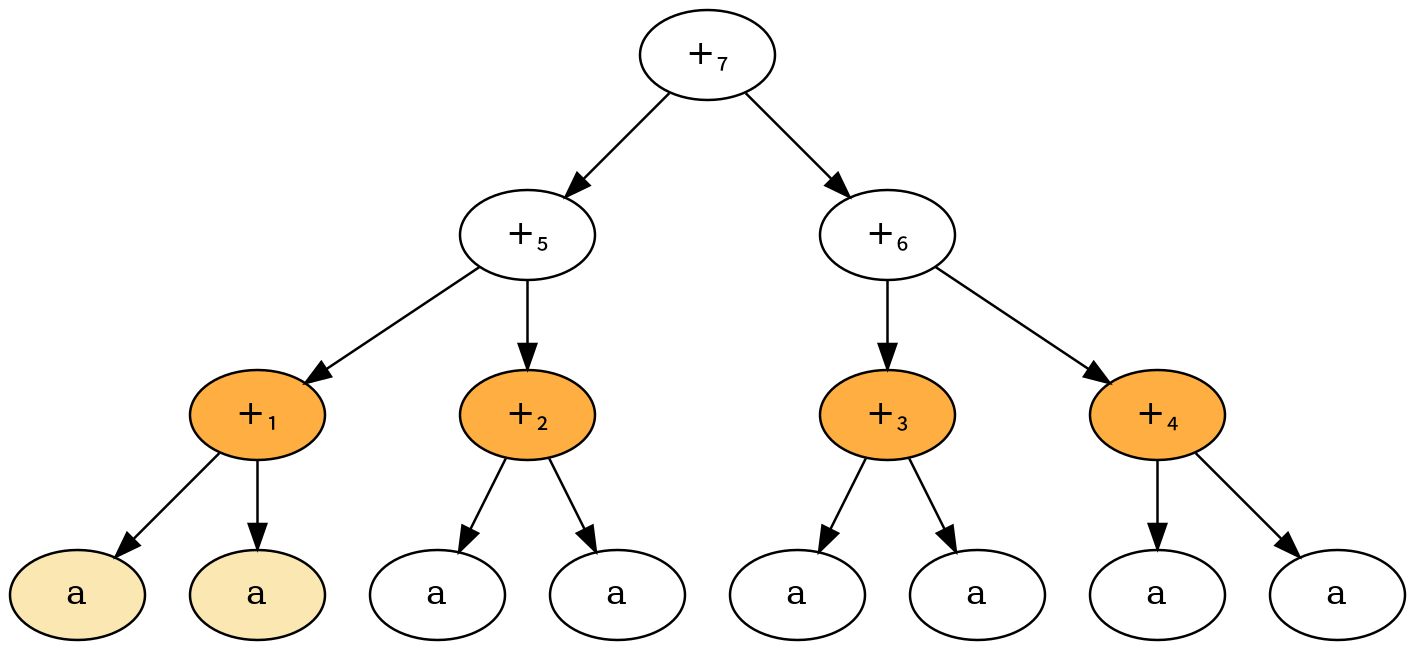
\includegraphics[height=4cm]{.dot/fold-power-2.png}
\end{center}

Evaluating \(a + a\) always yields the same result. So there is no point in
repeating this calculation 4 times.
\end{frame}

\begin{frame}[label={sec:org728e415}]{Power in terms of Monoid}
\begin{center}
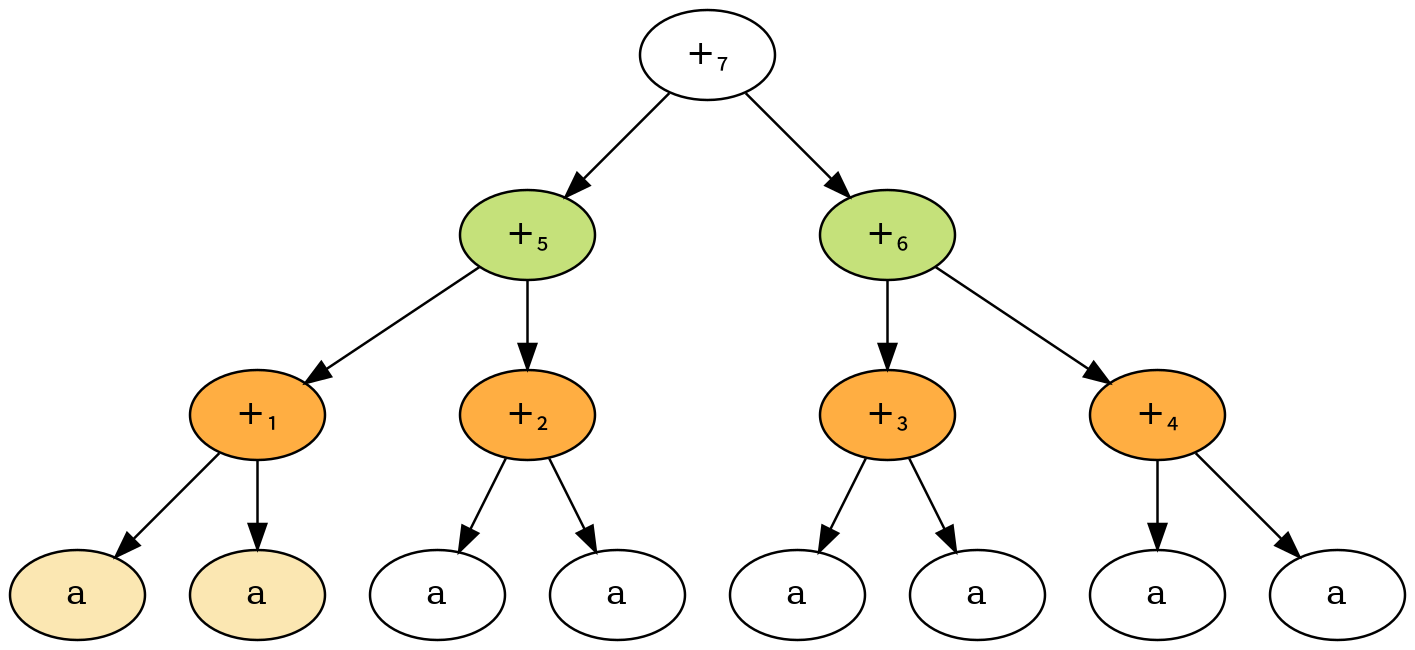
\includegraphics[height=4cm]{.dot/fold-power-3.png}
\end{center}

The same thing with the upper level. In this particular example, we can avoid 4
operations out of 7. In general, this optimisation leads to the result in \(\log
n\) operations.
\end{frame}

\begin{frame}[label={sec:org2b0cf96},fragile]{Power in terms of Monoid}
 All this means that we can define a function \texttt{power}:

\begin{minted}[]{scala}
def power[A: Monoid](a: A, n: Int): A = {
  ???
}
\end{minted}
\end{frame}

\begin{frame}[label={sec:orga8425c5}]{Back to Fibonacci}
Fibonacci number can be defined in a different way.

\begin{equation*}
  \begin{pmatrix}
    F_{n+1} & F_n \\
    F_n & F_{n-1}
  \end{pmatrix} =
  \begin{pmatrix}
    1 & 1 \\
    1 & 0
  \end{pmatrix} ^ n
\end{equation*}

\pause

\begin{itemize}
\item The Fibonacci number can be calculated using square nonnegative matrix
multiplication.
\item Square nonnegative matrices form Monoid with multiplication.
\item So we can put parentheses in a way we like it.
\end{itemize}
\end{frame}

\begin{frame}[label={sec:org3a427d2},fragile]{Time for work}
 \begin{itemize}
\item Open \texttt{wax.exercise.fibonacci} module.
\item Task is to implement monoid for \texttt{Matrix2x2}.
\item Run \texttt{MatrixMonoidSpecification} to test your instance.
\item Run \texttt{Main} object and compare benchmarking results of tail recursive and
matrix-based implementations.
\end{itemize}
\end{frame}

\begin{frame}[label={sec:org47c8c1d}]{Outcome}
\begin{itemize}
\item Just think about it.
\begin{itemize}
\item Giving any monoid we have a helper that allows us to efficiently calculate
\(a^n\).
\item This is not only because of the operations, but the laws (or so-called
properties) that come with these operations.
\item Monoids are everywhere around us. We deal with them every day, without even
noticing it.
\end{itemize}
\item You might forget how matrix multiplication works, but now you remember, right?
\end{itemize}
\end{frame}

\section*{Books}
\label{sec:org40621b6}

\begin{frame}[label={sec:orgfe35ece}]{Folds with Monoids}
\begin{itemize}
\item We already know that Monoids give us an ability to place parentheses in any
fashion.
\item We already saw that when it comes to folding the list of the same elements we
gain performance.
\item But what if the elements are not equal? Do we gain anything?
\end{itemize}

\pause
\begin{center}
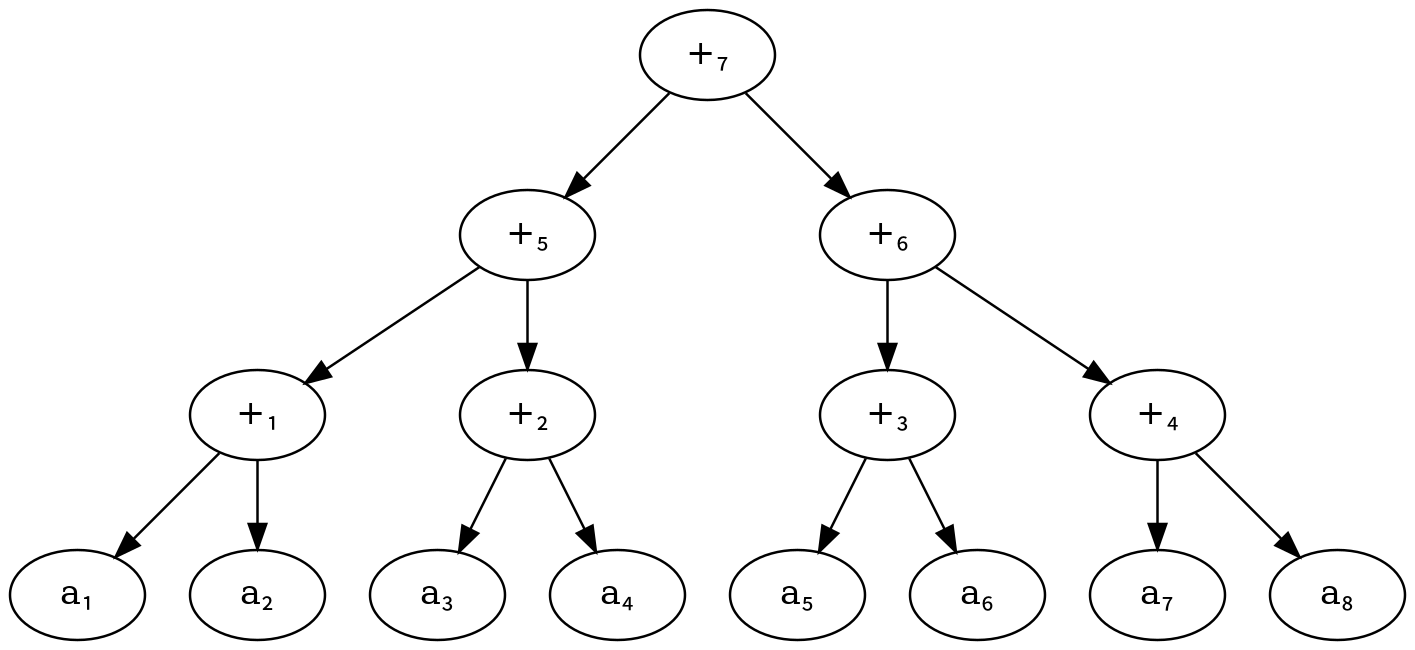
\includegraphics[height=4cm]{.dot/fold-parallel-1.png}
\end{center}
\end{frame}

\begin{frame}[label={sec:org8815553}]{Folds with Monoids}
\begin{center}
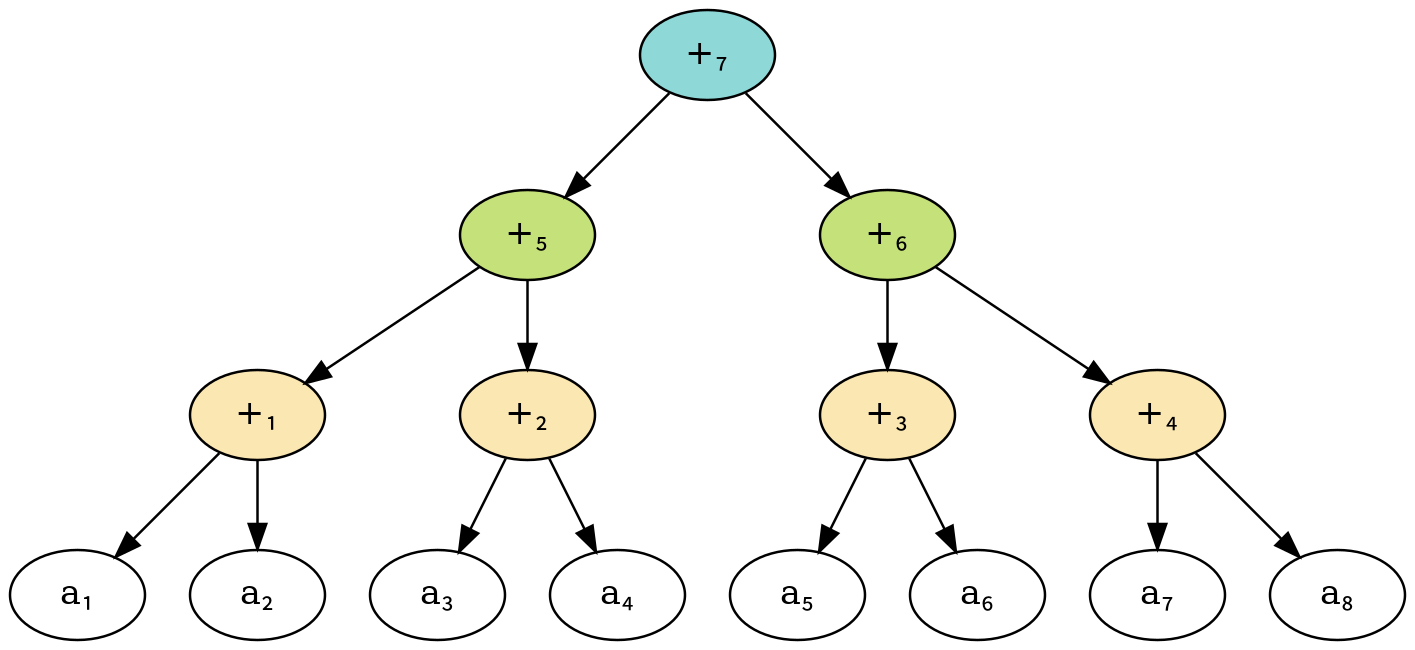
\includegraphics[height=4cm]{.dot/fold-parallel-2.png}
\end{center}

Every expression on each level does not depend on other expressions from the
same level, which means that we can evaluate them in parallel.
\end{frame}

\begin{frame}[label={sec:orgb57d589},fragile]{MapReduce}
 \begin{itemize}
\item Sometimes we have a collection of elements that don't form Monoid.
\item But we can transform (going ahead, \texttt{map}) them into something that is a Monoid
\begin{itemize}
\item Again, going ahead, this also can be done in parallel.
\end{itemize}
\item There is a strange accent, where people pronounce 'fold' as 'reduce'.
\item This is how we get the \texttt{mapReduce}.
\end{itemize}
\end{frame}

\begin{frame}[label={sec:org62535ad},fragile]{Getting the top used words from set of books}
 \begin{itemize}
\item Open \texttt{wax.exercise.mapreduce} module.
\item Task is to
\begin{itemize}
\item Implement monoid for \texttt{MapReduce.Result[A]}.
\item Implement the \texttt{job} function. Let's find the most used word among all the
books that is also longer than 4 symbols.
\end{itemize}
\item Books are located in the \texttt{resources} directory.
\item Use \texttt{allBooks} to load all available books or \texttt{authorBooks} to load all books
of specific author.
\begin{itemize}
\item \texttt{authorBooks("boris")} - you can use this author with small amount of text
to test your \texttt{job}.
\end{itemize}
\item Compare benchmark results.
\end{itemize}
\end{frame}

\section*{Logger}
\label{sec:orgeb59b7b}

\begin{frame}[label={sec:org7451bdd},fragile]{Things to note}
 \begin{itemize}
\item Functional programming is not about \texttt{Monads} and \texttt{IO}.
\begin{itemize}
\item Funny enough, first versions of Haskell were naked and no one dared to tell
the committee that \texttt{IO} is missing.
\end{itemize}
\item Functions matter.
\end{itemize}

\pause

\begin{itemize}
\item Can a function be monoid?
\end{itemize}
\end{frame}

\begin{frame}[label={sec:org35d0de7},fragile]{Let's start with some wrappers (pun intended)}
 \begin{itemize}
\item Suppose that we have some case class \texttt{Wrapper[A](value: A)}
\item Can it be a monoid?
\item Well, generally speaking, not! Because we know nothing about the type \texttt{A}.
\item But what if \texttt{A} is a monoid?
\end{itemize}

\pause

\begin{minted}[]{scala}
case class Wrapper[A](value: A)

object Wrapper {
  implicit def wrapperMonoid[A: Monoid]: Monoid[Wrapper[A]] = new Monoid[Wrapper[A]] {
    override def empty: Wrapper[A] = Wrapper(Monoid[A].empty)

    override def combine(x: Wrapper[A], y: Wrapper[A]): Wrapper[A] =
      Wrapper(Monoid[A].combine(x.value, y.value))
  }
}
\end{minted}
\end{frame}

\begin{frame}[label={sec:orge69e5ed},fragile]{Wrappers of monoids are monoids}
 \begin{itemize}
\item So IO can also be a monoid
\begin{minted}[]{scala}
def ioMonoid[A: Monoid]: Monoid[IO[A]] = ???
\end{minted}
\item Which means that we can combine IO actions (in some new sense).
\item Functions are wrappers (in some sense), so they also can be monoids
\begin{minted}[]{scala}
def functionMonoid[A, B: Monoid]: Monoid[Function[A, B]] = ???
\end{minted}
\item Which means that we can combine functions (in some new sense).
\end{itemize}
\end{frame}

\begin{frame}[label={sec:org39ab611},fragile]{Logger}
 \begin{itemize}
\item \texttt{Logger} is basically a function from \texttt{String} to \texttt{IO[Unit]}.
\begin{minted}[]{scala}
type Logger = String => IO[Unit]
\end{minted}
\item \texttt{Unit} forms a monoid.
\item So \texttt{IO[Unit]} forms a monoid.
\item So \texttt{String => IO[Unit]} forms a monoid.
\item So \texttt{Logger} forms a monoid.
\item So we can combine loggers
\begin{itemize}
\item \texttt{combine(fileLogger, consoleLogger)} - logs both into file and to console
\end{itemize}
\end{itemize}
\end{frame}

\begin{frame}[label={sec:org9d177d0},fragile]{Logger}
 \begin{itemize}
\item Open \texttt{wax.exercise.logging} module
\item Task is to implement monoid for \texttt{IO[Logger]}
\item Have fun!
\end{itemize}
\end{frame}

\section*{Recap}
\label{sec:org440002f}

\begin{frame}[label={sec:orgfcd535d},fragile]{Recap (recup?)}
 \begin{itemize}
\item Semigroup is something with means of combining these somethings.
\item Monoid is semigroup that also has neutral element that doesn't affect a combination.
\item Associativity is a powerful property giving us an ability to solve some tasks.
\begin{itemize}
\item \(a^n\) in \(\log n\)
\item \texttt{mapReduce}
\end{itemize}
\item Monoids are everywhere. They act like a plague, once something forms a monoid,
something else also begins to form a monoid.
\item We want some rest after a long session of workshop.
\end{itemize}
\end{frame}

\begin{frame}[label={sec:org0b21961}]{Questions?}
\centerline{\huge $\epsilon \rho \omega \tau \eta \sigma \eta$?}
\end{frame}

\begin{frame}[label={sec:org54dd883}]{Thank you very much!}
\centerline{\huge We hope you enjoyed this session.}
\end{frame}
\end{document}
